\documentclass[9pt, aspectratio=169]{beamer}

\usetheme{metropolis}
\setbeamertemplate{itemize items}{\faAngleRight}

\metroset{titleformat=smallcaps,block=fill,numbering=counter,progressbar=frametitle,sectionpage=none}
\setbeamersize{text margin left=5mm,text margin right=5mm} 
% %%%%%%%%%%%%%%%%%%%%%%%%%%%%%%%%%%%%%%%%%%%%%%%%%%%%%%%%%%%%%%%%%%%%%%%%%%%%%%
% \embedvideo{<poster or text>}{<video file (MP4+H264)>}
% \embedvideo*{...}{...}                     % auto-play
%%%%%%%%%%%%%%%%%%%%%%%%%%%%%%%%%%%%%%%%%%%%%%%%%%%%%%%%%%%%%%%%%%%%%%%%%%%%%%

\usepackage[bigfiles]{pdfbase}
\ExplSyntaxOn
\NewDocumentCommand\embedvideo{smm}{
  \group_begin:
  \leavevmode
  \tl_if_exist:cTF{file_\file_mdfive_hash:n{#3}}{
    \tl_set_eq:Nc\video{file_\file_mdfive_hash:n{#3}}
  }{
    \IfFileExists{#3}{}{\GenericError{}{File~`#3'~not~found}{}{}}
    \pbs_pdfobj:nnn{}{fstream}{{}{#3}}
    \pbs_pdfobj:nnn{}{dict}{
      /Type/Filespec/F~(#3)/UF~(#3)
      /EF~<</F~\pbs_pdflastobj:>>
    }
    \tl_set:Nx\video{\pbs_pdflastobj:}
    \tl_gset_eq:cN{file_\file_mdfive_hash:n{#3}}\video
  }
  %
  \pbs_pdfobj:nnn{}{dict}{
    /Type/RichMediaInstance/Subtype/Video
    /Asset~\video
    /Params~<</FlashVars (
      source=#3&
      skin=SkinOverAllNoFullNoCaption.swf&
      skinAutoHide=true&
      skinBackgroundColor=0x5F5F5F&
      skinBackgroundAlpha=0
    )>>
  }
  %
  \pbs_pdfobj:nnn{}{dict}{
    /Type/RichMediaConfiguration/Subtype/Video
    /Instances~[\pbs_pdflastobj:]
  }
  %
  \pbs_pdfobj:nnn{}{dict}{
    /Type/RichMediaContent
    /Assets~<<
      /Names~[(#3)~\video]
    >>
    /Configurations~[\pbs_pdflastobj:]
  }
  \tl_set:Nx\rmcontent{\pbs_pdflastobj:}
  %
  \pbs_pdfobj:nnn{}{dict}{
    /Activation~<<
      /Condition/\IfBooleanTF{#1}{PV}{XA}
      /Presentation~<</Style/Embedded>>
    >>
    /Deactivation~<</Condition/PI>>
  }
  %
  \hbox_set:Nn\l_tmpa_box{#2}
  \tl_set:Nx\l_box_wd_tl{\dim_use:N\box_wd:N\l_tmpa_box}
  \tl_set:Nx\l_box_ht_tl{\dim_use:N\box_ht:N\l_tmpa_box}
  \tl_set:Nx\l_box_dp_tl{\dim_use:N\box_dp:N\l_tmpa_box}
  \pbs_pdfxform:nnnnn{1}{1}{}{}{\l_tmpa_box}
  %
  \pbs_pdfannot:nnnn{\l_box_wd_tl}{\l_box_ht_tl}{\l_box_dp_tl}{
    /Subtype/RichMedia
    /BS~<</W~0/S/S>>
    /Contents~(embedded~video~file:#3)
    /NM~(rma:#3)
    /AP~<</N~\pbs_pdflastxform:>>
    /RichMediaSettings~\pbs_pdflastobj:
    /RichMediaContent~\rmcontent
  }
  \phantom{#2}
  \group_end:
}
\ExplSyntaxOff
%%%%%%%%%%%%%%%%%%%%%%%%%%%%%%%%%%%%%%%%%%%%%%%%%%%%%%%%%%%%%%%%%%%%%%%%%%%%%%

\usepackage{fontspec,minted}
\usepackage[scale=1]{ccicons}
\usepackage{metalogo}
\usepackage{xcolor,colortbl}
\usepackage{multicol,multirow,booktabs}
\usepackage{appendixnumberbeamer}
\usepackage{graphicx}
\usepackage{bm}
\usepackage{fontawesome}
\usepackage{csquotes}
\usepackage[backend=biber, natbib, sorting=nyt, doi=true, url=false, url=false, isbn=false, maxbibnames=10]{biblatex}
\addbibresource{../../utils/refs.bib}

\usepackage[spanish]{babel}
\usepackage{mathtools}
\usefonttheme{professionalfonts}
\usepackage{textcomp}

\setsansfont[BoldFont={Iwona Bold}, Numbers={Lining, Proportional}]{Iwona Light}
% \setmathsfont(Digits)[Numbers={Lining, Proportional}]{Fira Sans Light}
\setmonofont[Scale=MatchLowercase]{DejaVu Sans Mono}

\setbeamercolor{alerted text}{fg=red,bg=black!2}
\setbeamercolor{progress bar}{fg=red,bg=red!2}
\setbeamertemplate{itemize item}{\faCaretRight}
\setbeamertemplate{itemize subitem}{ \faAngleRight}
\setbeamertemplate{blocks}[shadow=false]
\setbeamercolor{block title}{bg=black!30,fg=red}
\setbeamercolor{block body}{bg=black!20,fg=black}
 
\usepackage{gensymb,amssymb}
\usepackage{upquote}
\usepackage{algpseudocode}
\algrenewcommand\algorithmicrequire{\textbf{Requiere}}
\algrenewcommand\algorithmicensure{\textbf{Devuelve}}
%\setbeamertemplate{blocks}[rounded][shadow=false]
\setbeamertemplate{blocks}[shadow=false]

\newcommand{\cx}{\column{0.5\textwidth}}
\newcommand{\cw}[1]{\column{#1\textwidth}}

\author{Manuel Carlevaro}
\date{{\tiny Departamento de Ingeniería Mecánica \\[-1em]
             Grupo de Materiales Granulares - UTN FRLP \\
        \faEnvelope{} manuel.carlevaro@gmail.com \- $\cdot$ \- \faTwitter{} @mcarlevaro}}
\institute{
  \vspace{6em}
  \centering
  {\tiny
  Cálculo Avanzado \enspace • \enspace 2022 \\
    \faLinux \- $\cdot$ \- \fontspec{TeX Gyre Pagella}\XeLaTeX \- $\cdot$ \- \ccbysa }
}

%% Operadores
\DeclareMathOperator{\sen}{sen}
\DeclareMathOperator{\sign}{sign}
\newcommand{\T}[1]{\underline{\bm{#1}}}
\DeclareMathOperator{\Tr}{Tr}

\usepackage{hyperref}
\hypersetup{
    colorlinks,
    citecolor=blue,
    filecolor=black,
    linkcolor=blue,
    urlcolor=blue
}
\urlstyle{same}

%% Códigos
\usepackage{minted}
\newminted[cpp]{cpp}{linenos,fontsize=\footnotesize,frame=lines,numbersep=4pt}
\newmintedfile[cppcode]{cpp}{linenos,fontsize=\footnotesize,frame=lines,numbersep=4pt}
\newcommand{\mic}[1]{\mintinline{C++}{#1}}

\newminted[py]{python}{linenos,fontsize=\footnotesize,frame=lines,numbersep=4pt}
\newminted[pyc]{pycon}{linenos,fontsize=\footnotesize,frame=lines,numbersep=4pt} % Consola de Python
\newminted[ipy3]{ipython3}{linenos,fontsize=\footnotesize,frame=lines,numbersep=4pt} % Consola de iPython3
\newmintedfile[pycode]{python}{linenos,fontsize=\footnotesize,frame=lines,numbersep=4pt}

\newmintedfile[makef]{basemake}{linenos,fontsize=\footnotesize,frame=lines,numbersep=4pt}
\definecolor{bg}{RGB}{22,43,58}
\newminted[shell]{console}{linenos=false,fontsize=\footnotesize,breaklines=true, frame=single} % Linea de comandos
\renewcommand\listingscaption{Código}

\makeatletter
\AtBeginEnvironment{minted}{\dontdofcolorbox}
\def\dontdofcolorbox{\renewcommand\fcolorbox[4][]{##4}}
\makeatother

% uso:
% Ejemplo de uso explícito:
% \begin{py}
% >>> list("abcd")
% ['a', 'b', 'c', 'd']
% \end{py}
% 
% Ahora ejemplo de código en file:
% \pycode{Chapters/intro/code/hola.py}
% 
% También se puede poner un sector del file:
% \pycode[firstline=6, lastline=7]{Chapters/intro/code/hola.py}
% 
% También se puede poner código \textit{inline}: \mip{print('¡Hola mundo!')} y en una sola línea:
% \slp|if __name__ == '__main__')|
% 
% Por último, se puede poner el código en un entorno \textit{float}, esto es, como las tablas y las figuras, con un caption y un label para luego hacer referencias, como por ejemplo al Código \ref{code:hola}.


\usepackage{tikz}
\usetikzlibrary{shapes,shadows,arrows,positioning,matrix,chains,backgrounds,fit}

\tikzset{
    %Define standard arrow tip
    >=stealth',
    %Define style for boxes
    obj/.style={
           rectangle,
           rounded corners,
           draw, very thick,
           text width=10em, fill=green!20,
           minimum height=2em,
           text centered, drop shadow},
    proc/.style={
	    rectangle, rounded corners,
	    draw,fill=red!50,very thick,
	    text width=8em,minimum height=2em,
	    text centered, drop shadow},
    % Define arrow style
    pil/.style={
           ->,
           thick,
           shorten <=2pt,
           shorten >=2pt,}
}

\setbeamertemplate{bibliography item}{%
  \ifboolexpr{ test {\ifentrytype{book}} or test {\ifentrytype{mvbook}}
    or test {\ifentrytype{collection}} or test {\ifentrytype{mvcollection}}
    or test {\ifentrytype{reference}} or test {\ifentrytype{mvreference}} }
    {\setbeamertemplate{bibliography item}{\faBook}}
    {\ifentrytype{online}
            {\setbeamertemplate{bibliography item}{\faGlobe}}
   {\setbeamertemplate{bibliography item}{\faFileText}}}%
  \usebeamertemplate{bibliography item}}

\defbibenvironment{bibliography}
  {\list{}
     {\settowidth{\labelwidth}{\usebeamertemplate{bibliography item}}%
      \setlength{\leftmargin}{\labelwidth}%
      \setlength{\labelsep}{\biblabelsep}%
      \addtolength{\leftmargin}{\labelsep}%
      \setlength{\itemsep}{\bibitemsep}%
      \setlength{\parsep}{\bibparsep}}}
  {\endlist}
  {\item}
\newcommand{\bcite}[1]{\citeauthor{#1}, \citetitle{#1} (\citeyear{#1})}


\title{Serie y Transformada de Fourier}
\subtitle{Funciones ortogonales. Series de Fourier. Ejemplos}


\begin{document}
\maketitle

\begin{frame}{ Funciones ortogonales }
\begin{columns}[t]
\cw{0.3}
Secuencia infinita $\{\phi_n(x)\}$ integrable en $[a, b]$ y
\[ \int_a^b \phi_i(x) \phi_j(x) \, dx = 0, \quad i \neq j \]

Supongamos que existe
\[ \int_a^b f(x) \, dx \]
y
\[ f(x) = \sum_{n = 1}^{\infty} c_n \phi_n(x) \]
\[c_3 = \color{red}{?} \]
\[ f(x) \phi_3(x) = \sum_{i = 1}^{\infty} c_n \phi_n(x) \phi_3(x) \]
\cw{0.3} \vspace{-1.5em}
\begin{multline*}
\int_a^b f(x) \phi_3(x) \, dx = \\
\int_a^b \sum_{i = 1}^{\infty} c_n \phi_n(x) \phi_3(x) \, dx = \\
\sum_{i = 1}^{\infty} \int_a^b c_n \phi_n(x) \phi_3(x) \, dx = \\
c_3 \int_a^b \phi_3^2(x) \, dx
\end{multline*}
\begin{equation}
c_k = \frac{\int_a^b f(x) \phi_k(x) \, dx}{\int_a^b \phi_k^2(x) \, dx} 
\label{eq:ck}
\end{equation}
\begin{definition}
Producto interno:
\[ \langle \phi_i, \phi_j \rangle = \int_a^b \phi_i(x) \phi(j)(x) \, dx \]
\end{definition}
\cw{0.3}
Con $c_k$ definida por \eqref{eq:ck}:
\[f(x) \sim \sum_{n = 1}^{\infty} c_n \phi_n(x) = F(x) \]
$F(x)$ es la \textbf{representación de Fourier} de $f(x)$ con respecto de $\{\phi_n(x)\}$.

Se puede demostrar:
\begin{multline*}
    \int_a^{b} \left[ f(x) - \sum_{k = 1}^n c_k \phi_k(x) \right]^2 \, dx \leq \\
    \int_a^{b} \left[ f(x) - \sum_{k = 1}^n d_k \phi_k(x) \right]^2 \, dx 
\end{multline*}
\end{columns}
\end{frame}

\begin{frame}
\begin{columns}[t]
\cx
\textbf{Caso especial:}
\begin{multline*}
\{1, \cos x, \cos 2x, \cos 3x, \cdots, \\
\sen x, \sen 2x, \sen 3x,  \cdots \} 
\end{multline*}
ortogonales en $[-\pi, \pi]$.

Por ejemplo:
\begin{multline*}
\int_{-\pi}^{\pi} \cos mx \, \cos nx \, dx = \\
\frac{1}{2} \int_{-\pi}^{\pi} [\cos(m + n) x + \cos(m - n) x] \, dx = \\
\frac{1}{2} \left[ \frac{\sen(m + n) x}{m + n} + \frac{\sen(m-n) x}{m - n} \right]_{x = -\pi}^{\pi} \\
= 0
\end{multline*}
\cx
\textbf{Resultado clave:}

Supongamos que $f(x)$ sea suave a tramos en $[-\pi, \pi]$, y que
\[ F(x) = \sum_{n = 0}^{\infty} a_n \cos nx + \sum_{n = 1}^{\infty} b_n \sen nx \]
es la representación de Fourier de $f(x)$. Entonces, para $x \in [-\pi, \pi]$:
\[ F(x) = \frac{f(x^+) + f(x^-)}{2} \]

\begin{exampleblock}{Ejemplo:}
    \begin{equation*}
        f(x) = \begin{cases}
            -1, &-\pi \leq x < 0 \\
            \phantom{-}1, &0 \leq x < \pi
        \end{cases}
    \end{equation*}
\end{exampleblock}
\end{columns}
\end{frame}

\begin{frame}
\begin{columns}[t]
\cx
\begin{align*}
F(x) &= \frac{4}{\pi} \sum_{n \text{ par}}^{\infty} \frac{\sen nx}{n} =  \frac{4}{\pi} \sum_{n = 0}^{\infty} \frac{\sen (2 n + 1) x}{2 n + 1}\\
     &= \frac{4}{\pi} \left( \sen x + \frac{\sen 3x}{3} + \frac{\sen 5 x}{5} + \cdots \right)
\end{align*}
Primeros dos términos:
\begin{center}
    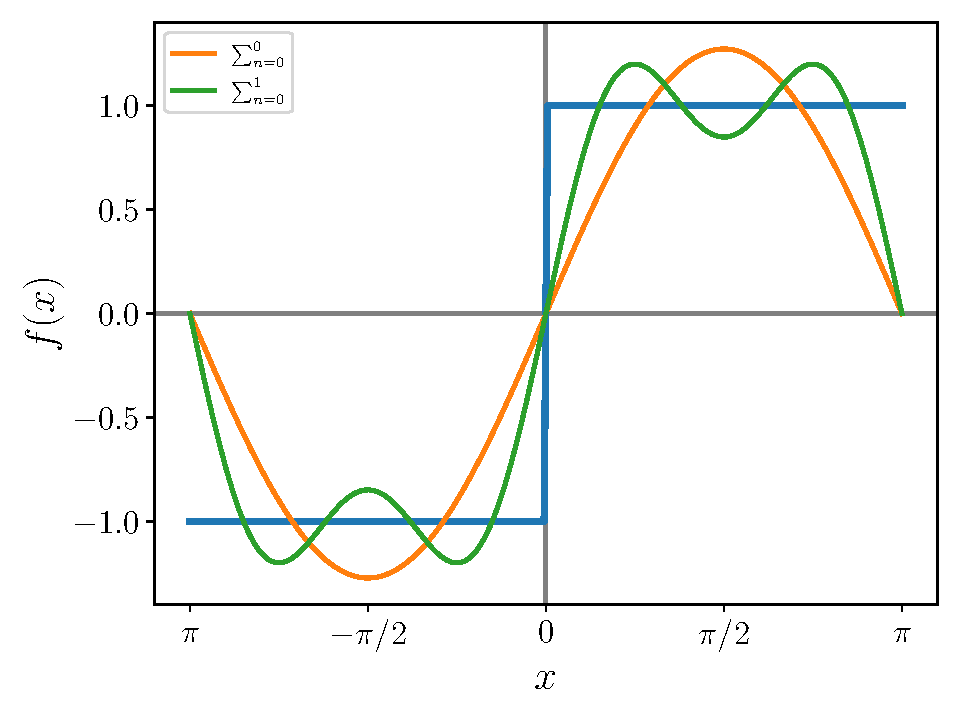
\includegraphics[scale=0.45]{figs/step-01.pdf}
\end{center} \pause

\cx
Agregando más términos:
\begin{center}
\only<2>  { 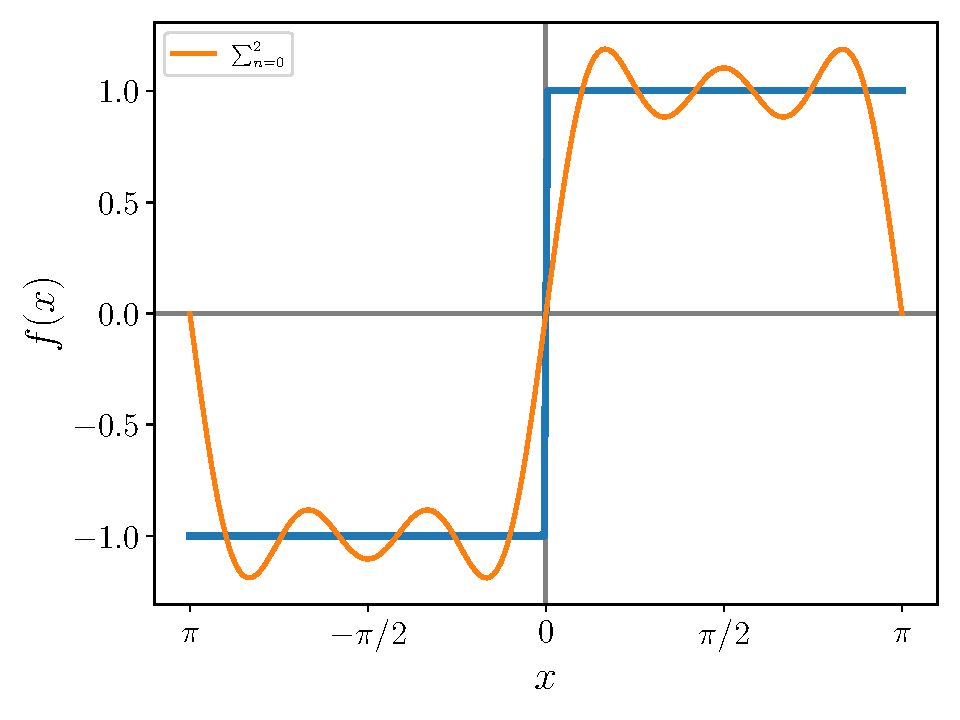
\includegraphics[scale=0.45]{figs/step-2.pdf} }
\only<3>  { 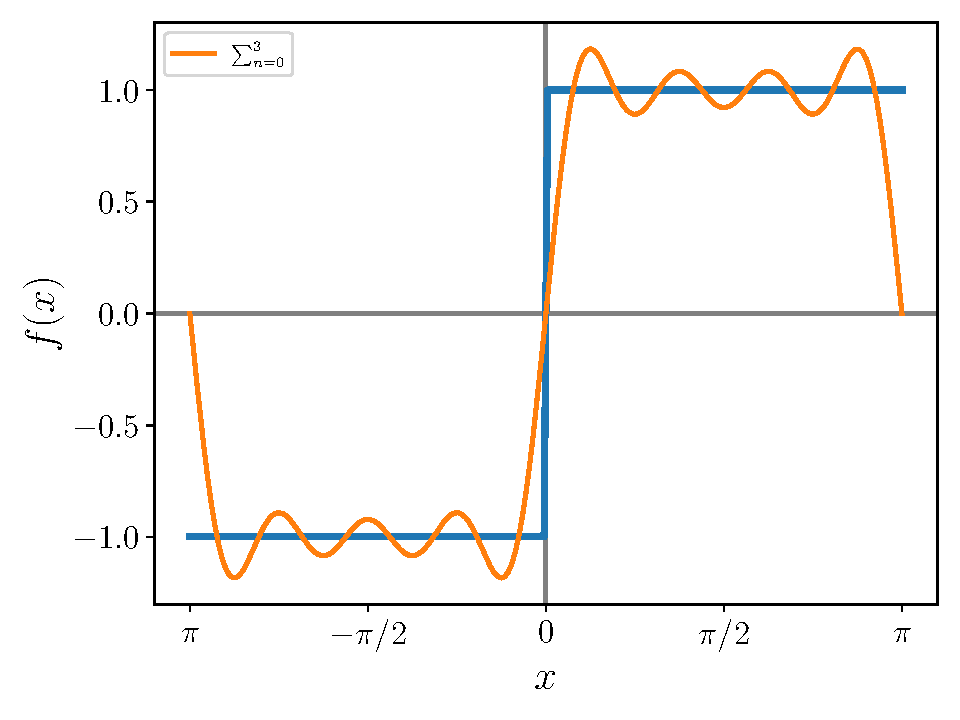
\includegraphics[scale=0.45]{figs/step-3.pdf} }
\only<4>  { 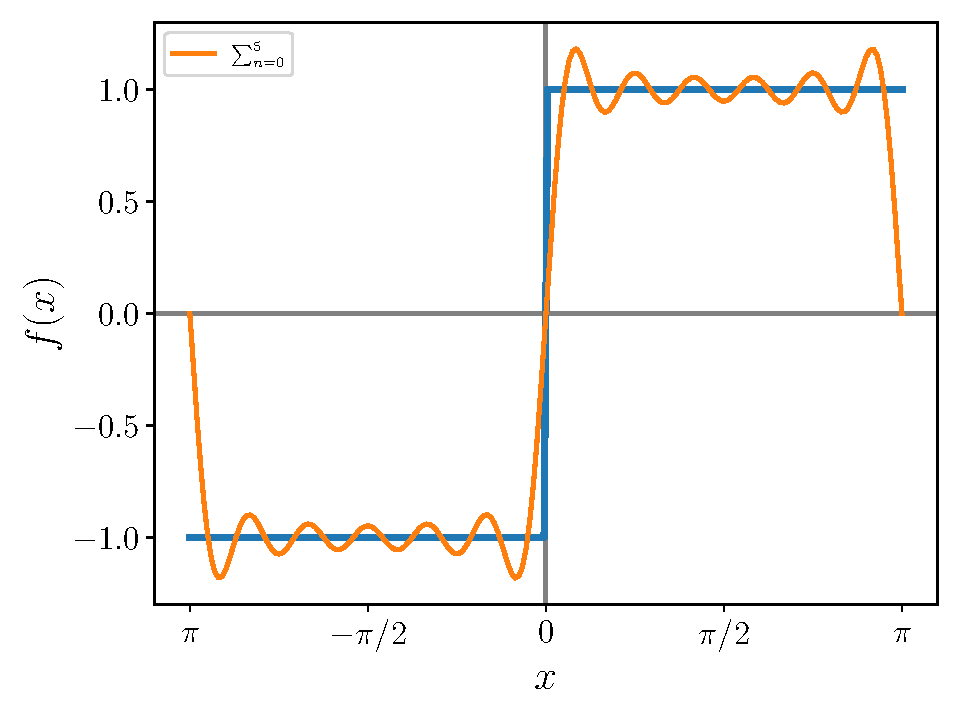
\includegraphics[scale=0.45]{figs/step-5.pdf} }
\end{center}

\only<2> {\[F_2(x) = \frac{4}{\pi} \left( \sen x + \frac{\sen 3x}{3} + \frac{\sen 5 x}{5} \right) \]}
\only<3> {\[F_3(x) = \frac{4}{\pi} \left( \sen x + \frac{\sen 3x}{3} + \frac{\sen 5 x}{5}  + \frac{\sen 7 x}{7}\right) \]}
\only<4> {\[F_5(x) = \frac{4}{\pi} \left( \cdots + \frac{\sen 9x}{9} + \frac{\sen 11 x}{11}  + \frac{\sen 13 x}{13}\right) \]}
\end{columns}
\end{frame}

\begin{frame}
\begin{columns}[t]
\cx
\textbf{Otro ejemplo:}
\begin{align*}
f(x) &= |x|, \quad -\pi < x < \pi \\
F(x) &= \frac{\pi}{2} - \frac{4}{\pi} \sum_{n \text{ impar}}^{\infty} \frac{\cos nx}{n^2}
\end{align*}

\begin{center}
    \only<1> {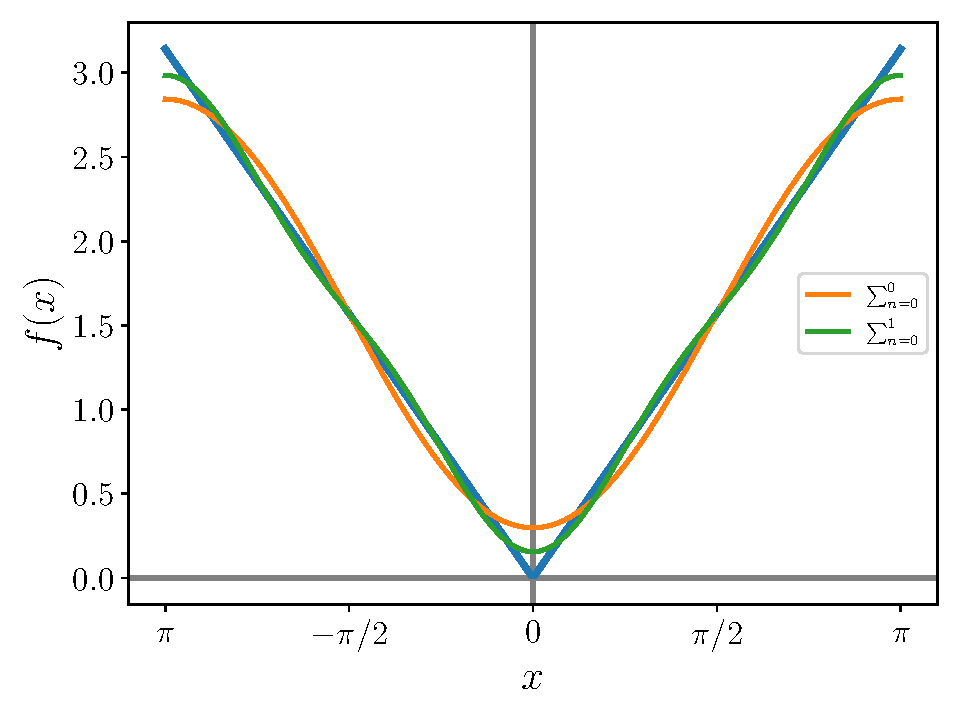
\includegraphics[scale=0.45]{figs/abs-01.pdf}}
    \only<2-> {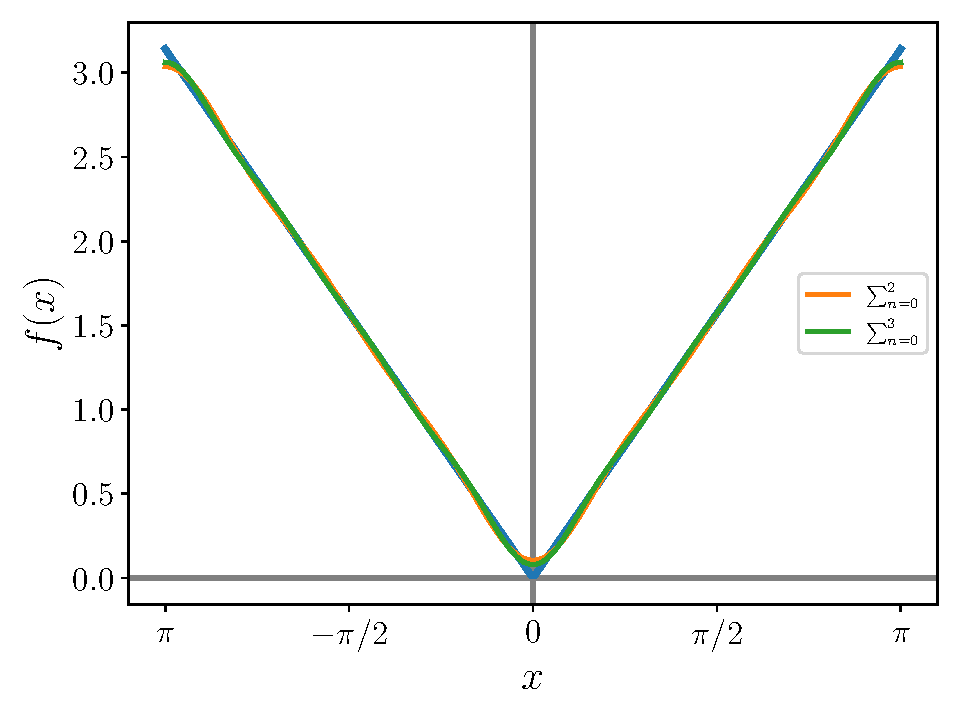
\includegraphics[scale=0.45]{figs/abs-23.pdf}}
\end{center}
\pause 

\cx
\textbf{Comparación con serie de potencias:}
\begin{multline*}
e^x = \sum_{n = 0}^{\infty} \frac{x^n}{n!} \\
= 1 + x + \frac{x^2}{2} + \frac{x^3}{6} + \frac{x^4}{24} + \frac{x^5}{120} + \cdots
\end{multline*}
\begin{center}
    \only<3> {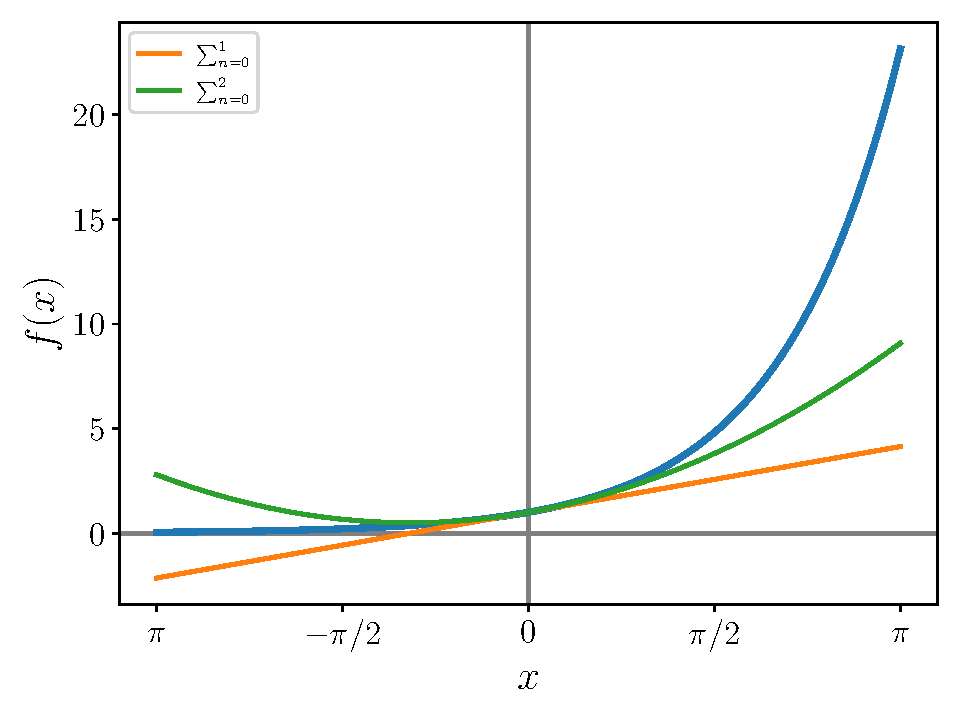
\includegraphics[scale=0.45]{figs/pot-12.pdf}}
    \only<4> {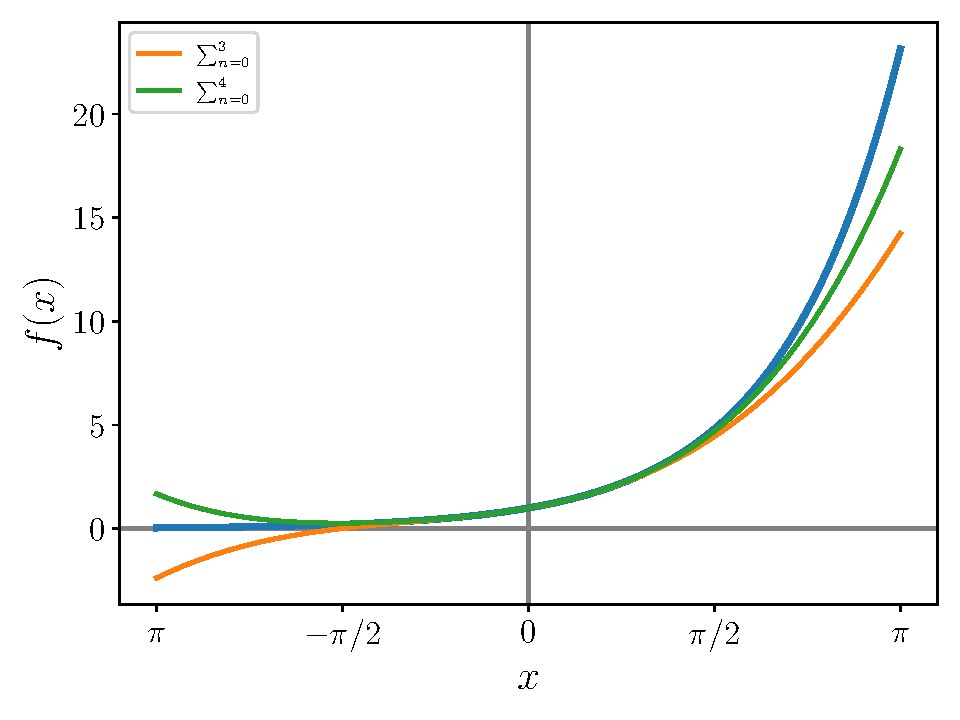
\includegraphics[scale=0.45]{figs/pot-34.pdf}}
\end{center}
\end{columns}

\end{frame}

\section*{Bibliografía}
\begin{frame}[allowframebreaks]{Lecturas recomendadas}
\begin{itemize}
 \item \fullcite{kreyszig2011}. Capítulo 11 (11.1 -- 11.6).
 \item \fullcite{oneil2012es}. Capítulo 2.
 \item \fullcite{stroud2020}. Capítulos 7 y 8.
\end{itemize}
\end{frame}


\end{document}

